\documentclass[10pt,a4paper]{report}
\setlength\parindent{0pt}
\usepackage[latin1]{inputenc}
\usepackage{amsmath}
\usepackage{amsfonts}
\usepackage{minibox}
\usepackage{amssymb}
\usepackage{graphicx}
\usepackage{listings}
\usepackage{wrapfig}
\usepackage{fullpage}

\author{Sander Demeester}
\title{Data compression - Burrows-Wheeler}
\begin{document}
\maketitle
\begin{abstract}
In dit verslag leg ik kort uit welke algoritmes ik heb ge\"implementeerd en op welke manier ik dit heb gedaan. Ik zal ook kort toelichten hoe mijn code is gestructureerde en welke ontwikkelings beslissingen ik heb genomen en waarom.\\

Daarna wat het effect is van de verschillende algoritmes op voorbeeld test bestanden en tijdsmetingen van de verschillende implementaties van deze algoritmen. 
\end{abstract}
\section*{Beschrijving implementatie}
\subsection*{main.c}
Om te kunnen kiezen tussen de verschillende implementaties en deze op een elegante manier te laten uitvoeren adhv een parameter die wordt meegeggeven met het programma heb ik gebruik gemaakt van functie pointers. Deze functie pointer zitten in een struct (compressie\_argument) samen met een value die ze uniek identificeert. Deze value wordt mee in de header geschreven tijdens het encoderen om daarna te worden ingelezen door het decoderen in de variabel compressie\_function\_pointer. Een simpele for-lus zal daarna het correct algoritme uitvoeren op basis van deze variabel.\\

Het bestand wordt hier ingelezen en verdeeld in blokken van grote $\text{blocksize}*1024$ om daarna in seqentie te worden verwerkt door het gespecificeerde algoritme, de stub voor al deze algoritmes bevind zich in de source-file "compressie\_methode.c".
\subsection*{compressie\_methode.c}
Deze source file bevat de stub voor het encoderen en decoderen van de verschilende algoritmes, het werk wordt via de struct compressie\_argument gedelegeert naar deze source file.\\

Algoritme 1 is standaard huffman in combinatie met move to front toegepaste op een Burrows-Wheeler vector. Burrows-Wheeler wordt altijd eerst uitgevoerdt vanuit main.c, testen hebben aangeduid dat dit bijna altijd resulteert in een optimalere tekst voor compressie, lostaand welke compresie algoritme nadien wordt gebruikt. Aan alle functies in \emph{compressie\_methode.c} wordt een argument meegeven die zegt of de input buffer al is gesegmenteerd of nog gesegmenteerd moet worden.\\

Het door- en terug geven van resulaten aan deze stub code gebeurdt voor het encoderen via de zelfde buffer als waar de input zit, voor het decoderen wordt een speciale struct gebruikt. Tijdens het alloceren van geheugen wordt hiermee rekening gehouden.

Voor het terug geven van het resultaat bij het decoderen is er een speciale struct voorzien, nl ("huffman\_decode\_result") en ("lz77\_result"). 
\subsection*{bw.c}
Elke implementatie van een algoritme heeft de mogelijkheid individueel te worden getest, dit is om eenvoudiger bugs op te sporen en indivuduele tijdsmeetingen te doen, via algoritme parameter "0" is het mogelijk om enkel Burrows-Wheeler toe te passen op een tekst.\\

Burrows-Wheeler is een manier om gegeven een tekst $t$ deze om te zetten naar een tekst $t^{'}$ waar $t^{'}$ beter is gestructureerd voor compressie met bv, huffman. Dit wordt gedaan door de tekst te zien als een matrix $M$ en deze lexografish te sorteren en de laaste kolom te zien als onze Burrows-Wheeler vector. Deze vector bevat als componenten de prefixen voor de eerste kolom vector van de matrix $M$. We merken op dat het optimaal zou zijn om de eerste kolom als Burrows-Wheeler vector te gebruiken, helaas is het niet mogelijk om enkel uit deze vector de originele tekst terug te constru\"en. Dit is wel mogelijk al we de laaste kolom van $M$ gebruiken (omdat $M$ een cyclische permutatie is). Het is belangrijk om in te zien dat de laaste kolom gebruiken dan wel niet de meest optimale manier is, het is nog altijd een prima transformatie! Hierbij is het belangrijk om te zien wat Burrows-Wheeler doet en op welke input teksten het een positief effect heeft. \\

We onderscheiden 2 soorten teksten. De eerste tekst is een random tekst, eventueel gemaakt met /dev/urandom, of de output van een goed encryptie cijfer, zoals AES. De tweede tekst is een tekst uit de nederlandse taal. \\
Voor de eerste tekst geldt dat er geen verbanden zijn tussen de opeenvolgende bytes in de tekst. Dus wanneer we een lexografish orderning opleggen zal deze geen zinnevolle invloed hebben op de compresibiliteit van de tekst (nl, het aantal herhalingen van dezelfde bytes na elkaar). We hebben het hier niet over de compresibiliteit van de eerste kolom! Want deze zou dezelfde zijn voor een random tekst als voor een taalkundig gestructureede tekst, maar wel over de prefixen van de symbolen in de eerste kolom, nl de laatste kolom van $M$.

Als we dit vergelijken met de 2de soort tekst dan merken we wel op dat er een verband is tussen opeenvolgende bytes, bepaalde opeenvolging van bytes komen herhaaldelijk voor in een gegeven tekst. Als we nu hier een lexografish orderning opleggen zullen we zien de eerste kolom van $M$ terug alle suffixen bevat als van laatste kolom, het verschil is nu dat de componenten in de laatste kolom nu ook een prima compresibiliteit heeft omdat er een taalkundig verband is tussen de opeenvolgende bytes.

Om enkel de snelheid van Burrow-Wheeler te testen heb ik 20 random files aangemaakt met grote 1MiB tem 20Mib en deze laten encoderen met varierende blokgrotes, 1 tem 5KiB\\

De functie die de Burrows-Wheeler implementatie opstelt neemt als argument een \emph{bwt\_blok} van lente \emph{len} en maakt een array van lengte \emph{len} die als waarde de indexen heeft van \emph{bwt\_blok}, daarna zullen we \emph{bwt\_blok} kopieren naar \emph{bwt\_transformatie} omdat we de originele tekst zullen overschrijven met onze Burrows-Wheeler vector. We zullen de lijst met indexen beschouwen als een lijst van pointers in de \emph{bwt\_transformatie}. Deze ene lijst zullen we samen met de gebruiken als voorstelling van onze Burrows-Wheeler matrix. De manier waarop ik dit heb gedaan kan worden gezien aan het volgend stukje c-code die eenvoudig deze matrix uitprint:

\begin{lstlisting}
int i = 0;
  int j = 0;
  for(i=0; i < len; i++){
    for(j = 0; j < len; j++){
      printf("%c",*(&rij[(rij_index[i]+j) % len]));
    }
    printf("\n");
  }
\end{lstlisting}
Waar dus $(i,j)$ resp rij en kolom voorstellen en de elementen uit \emph{rij\_index} gebruiken als pointers in de rij die onze Burrows-Wheeler transformatie moet voorstellen. \\

Daarna zal een aangepaste versie van het quicksort sorteer algoritme worden gebruikt om de rij van indexen te sorteren adhv de waarden in de rij \emph{bwt\_transformatie}.\\

Het quicksort algoritme is lichtjes aangepast om correct te kunnen werken met de voorstelling van de Burrows-Wheeler transformatie, nl als er gelijke elementen zijn moeten kijken naar het volgende element in de huidige rij van deze matrix, dit is enkel maar bij het encoderen want bij het decoderen passen we een andere manier van elementen vergelijken toe. Er wordt gebruikt gemaakt van de volgende c-notatie om dit correct te laten gebeuren. 
\begin{lstlisting}
 while(*(&rij[(rij_index[links]+offset)%len]) == *(&rij[(rij_index[begin]+offset)%len]))
    {
    if(offset+1 == len) break;  
    offset = (offset+1) % len;
    }
	 
 if(*(&rij[(rij_index[links]+offset) % len]) > *(&rij[(rij_index[begin]+offset) % len]))
	 swap(&(rij_index[links]),&(rij_index[--rechts]));
 else
	 links++;	 
\end{lstlisting}
We houden een offset bij en maken terug gebruik van de modulo operator om naar het correct element te gaan dat wordt aangeduid door de pointer in \emph{rij\_index} waarop we dan de offset bijtellen om te kijken of deze volgende tekens duidelijk van elkaar verschillen.\\

Daarna gaan we met een simpele for-lus de laatste kolom nemen uit deze matrix en dit zal onze finale Burrows-Wheeler transformatie zijn. De laaste kolom uit een cyclische gepermuteerde matrix die door 1 rij wordt voorgestelt halen we op met de volende c-notatie:
\begin{lstlisting}
bwt_blok[i]= *(&bwt_transformatie[(rij_index[i-5]+(blocksize-1)) % blocksize]);
\end{lstlisting}
Voor het decoderen van een Burrows-Wheeler transformatie zijn de eerste 4 bytes de startpositie van onze vector, daarna maken we 2 rijen aan, \emph{sorted\_rij\_index} en \emph{bwt\_rij\_index}. De \emph{sorterd\_rij\_index} zal de lijst zijn die wordt gesorteerdt door quicksort op basis van de Burrows-Wheeler vector. De andere rij, \emph{bwt\_rij\_index} zal gewoon een lijst zijn met pointers naar de niet gesorteerde originele Burrows-Wheeler vector. \\

Nu maken we gebruik van het feit dat de Burrows-Wheeler matrix een cyclische permutatie is van een reeks tekst, en aangezien we als vector de laatste kolom van deze matrix hebben gebruikt weten we ook dat de eerste kolom van deze marix de prefix is voor de Burrows-Wheeler vector, nu omdat we een cyclische permutatie hebben weten dat het volgende element staat op de index in de originele lijst van niet gesorteerde lijst met pointers, waardoor het vinden van de volgende positie triviaal simpel wordt en de implementatie kan gewoon worden bekomen door simpele for-lus over de lengte van de vector.
\begin{lstlisting}
for(int i = 0; i < len; i++){
	start_pos = sorted_rij_index[bwt_rij_index[start_pos]];
}
\end{lstlisting}
Wat de volledige complexiteit voor het decoderen $O(2n + \log n)$ maakt.
\subsection*{move\_to\_front.c}
Met de \emph{Move to front}-methode proberen we het idee dat we proberen te bereiken met Burrows-Wheeler (nl, vaak voorkomende tekens samen te groeperen en lieft met zoon klein mogelijk index nummer). Move to front dit exact dit, het gaat gegeven een input string en een alfabet alle symbolen in de input string overlopen en de index van het huidige symbool opslaan en vooraan plaatsen in het alfabet. Dit zal tot gevolg hebben dat symbolen die vaak voorkomen in de input string zullen resulteren in een laag index positie nummer in het resultaat omdat deze tekens vaak vooraan blijven zitten in het alfabet.\\

Voor mijn implementatie heb ik gebruikt gemaakt van een dubbele cyclische gelinked lijst die als waardes een unsigned byte bijhoudt en een pointer naar het volgende en vorige element. De volledige  gelinked lijst heeft standaard als waardes die kunnen worden voorgesteld door 1 byte, nl 256 waarden.\\ 
Een simpele for-lus overloopt alle waardes in de input string en maakt daarin gebruik van een while lus die door de gelinked lijst loopt tot dat de gezochte waarde is gevonden in de gelinked lijst, er wordt een teller bijgehouden die kijkt wat de positie is van het gezocht symbool in de gelinked lijst en die wegschrijft.\\

Voor simpliciteit beschouwen we 2 gevallen in deze linkedlist, als het eerste element vooraan staat moet niks gebeuren (dit is het geval als c==0), in het andere geval verhangen we het gevonden element naar de eerste plaats.\\

Ook voor deze code heb ik een aparte unit test file gemaakt om te kunnen garanderen dat deze code correct werkt. 
\subsection*{huffman.c}
Deze source file bevat alle code die betrekking heeft op mijn implementatie van het standaard huffman algoritme. Het encoderen en decoderen van het algoritme is  ge\"emplementeerd in de zelfde functie, adhv een paramter kan worden beslist wat er moet worden uitgevoerd. \\

\subsubsection*{Encoderen}
Eerst wordt een frequentietabel gebouwde van bytes in de input\_string. Daarna gaan we 256 codewoorden aanmaken (van het type huffman\_codewoord). Deze codewoorden worden geindexeerd met de ascii waarden van de originele byte (de byte die ze voorstellen) en bevatten 2 velden, het aantal bits dat deze code bevat en de code zelf. Ook worden huffman\_toppen aangemaakt, deze toppen stellen de originele bytes voor die een freqentie hebben groter dan 0. Deze lijst van toppen zal worden gebruikt om de huffman code op te stellen. \\

In de hulp functie \emph{build\_huffman\_code} zullen deze toppen in omgekeerd sorteeerde volgorde worden overlopen (van lage frequentie naar hoge frequentie). 
$$(t_{0},t_{1},\cdots,t_{n-1},t_{n}) | w(t_{i}) < w(t_{i-1})$$
met $w(t)$ het frequentie gewicht van top $t$. We beschouwen de 2 elementen met de laagste frequentie, dit zijn $(t_{n-1},t_{n})$, deze bevatten een lijst van value (de eerste keer dat dit wordt uitgevoerd bevat elke top maar 1 value, voor de volgende iteraties zullen deze toppen meer values bevatten) die we gaan gebruiken als indexen in onze code tabel waar we bits gaan shiften. Voor $t_{n-1}$ bit "1", resp voor $t_{n}$ bit "0". In c-notatie:
\begin{lstlisting}
for(k = 0; k  < huffman_toppen[i-1]->aantal_elementen; k++){       
	code[(uint32_t)huffman_toppen[i-1]->value[k]]->code <<= 1; 
	code[(uint32_t)huffman_toppen[i-1]->value[k]]->code |= (1<<0);
	code[(uint32_t)huffman_toppen[i-1]->value[k]]->number_of_bits++;
\end{lstlisting}

Eenmaal dit is gedaan zullen we de 2 laagste toppen samenvoegen tot 1
We werken nog altijd met $(t_{n-1},t_{n})$. Het veld \emph{aantal\_elementen} zal de som van beide vleden \emph{aantal\_elementen} zijn van de 2 toppen, het gewicht (de frequentie) zal ook samen worden getelt en originele bytes die de toppen voorstelde zullen ook worden samengevoegd. Daarna zal deze nieuwe top een opwaarste perculatie maken tot dat zijn frequentie waarde net kleiner is dan de top boven hem in de lijst.\\

Er wordt uiteraardt geen nieuwe top aangemaakt maar top $t_{n-1}$ wordt herbruikt, dit wordt herhaalt tot er nog 1 top over is. \\

Daarna wordt de originele tekst gebruikt als indexen naar de code tabel en worden code-bits uit deze code geshift in een output buffer. Hierbij is het belangrijk dat de bit sequentie die is opgeslagen in de huffman codewoorden wordt omgedraaidt. De reden hiervoor is omdat we tijdens het encoderen zijn vertrokken bij de toppen met de laagste frequentie (de bladeren van onze huffman boom) en langzaam zijn we in aantal toppen geminderd opweg naar de top met de hoogste frequentie. Dus onze bit sequentie $b_{1},b_{2},\cdots,b_{k}$ voor een gegeven codewoord die is opgesteld door \emph{build\_huffmancode} heeft als MSB bit $b_{1}$ en stelt in het geval dat we deze voorbeeld code nemen het blad voor van de code. En het pad $p_{i}$ van blad naar wortel is in termen van bit sequentie niet het zelfde als pad $p_{j}$ waar zowel het zelfde blad als wortel voor beide padden de eind punten zijn. We mogen dus niet in deze volgorde onze coden versturen omdat de ontvanger niet correct de codewoorden zou interpreteren. \\

De code is slim genoeg om te merken hoeveel plaats er nog vrij is de huidige output byte en kan codewoorden opdelen zodat het aantal output bytes optimaal kan worden benut.
Daarna wordt een huffman header opgestelt die uit 12byte bestaat.\\
De eerste 4bytes is de lengte van het volledige huffman blok, incl de huffmancode en huffman frequentie  (zonder de header). 
De volgende 4 bytes is de lengte van de huffman code zelf. De laatste 4 bytes is de lengte van de huffman frequentie.\\

Bij elk huffman blok wordt ook de huffman frequentie doorgegeven. Elke frequentie blok heeft een lengte van 5 bytes, 4 bytes om het aantal voorkomens mee aan te duiden en 1 byte om het originele teken zelf voor te stellen. Enkel de frequenties voor niet 0 bytes worden opgenomen in deze huffman frequentie. Ik maak geen gebruik van relatieve frequenties omdat er gevallen zijn waar afronding van floating point getallen zou kunnen leiden tot verkeerde frequenties endus tot verkeerde codes bij het decoderen.\\
Daarna schrijven we alles ook in de zelfde volgorde weg, als laatste byte geven we nog mee hoeveel bits we hebben gebruikt als "padding" bij het maken van huffman code.
\subsubsection*{Decoderen}
Het decoderen verloopt voor het eerste deel gelijk met het encoderen. Eerst wordt adhv van de huffman frequentie de frequentie opgebouwd voor de verschillende originele bytes, en opnieuw wordt terug een lijst opgebouwd van huffman codewoorden. Dit keer zullen we een echte "boom" opstellen langswaar we tijdens het decoderen zullen wandelen tot we een blad tegenkomen met een waarde. We zullen tijdens het opstellen elk codewoord als een pad beschouwen langswaar we wandelen enz takken in onze boom defineren, aangezien elk codewoord uniek is zal ook elke wandeling uniek zijn endus zal de boom correct zijn.\\

Daarna wordt voor elke bit in de ontvangen huffman-code de boom doorlopen, en het resultaat opgeslagen in een output buffer. 
\subsection*{lz77.c}
Voor deel 2 van de opgave heb ik gekozen voor puntje 4, "Het kiezen van een eigen compressie algoritme". heb ik gekozen om lz77 te gebruiken waarvan de input is getransformeerdt met Burrows-Wheeler en de output wordt geencodeerdt met standaard huffman. \\

Een lz77 codewoord is van de vorm (p,l,x), waar de "p" staat voor de start van de langste een match in het sliding window, "l" staat voor de lengte van de match en "x" bevat de byte die volgt op de match.\\

Voor de implementatie maak ik gebruik van het concept "Match-pair", een match-pair is een return type voor de functie \emph{find\_longest\_string} en heeft de start positie en de lengte van de langste match terug die start in het sliding window. Daarnaast maak ik ook gebruik van 2 index variabelen die de start en het einde van het sliding window aanduiden.\\

Ik maak gebruik van het zoek string algoritme "Knuth-Morris-Pratt" dat lichtjes is aangepast om de langste match te vinden in het sliding window, ik beschrijf deze aanpassingen hier.\\

Beschouw een reeks van tekens:
$$(x_{0},x_{1},x_{2},\cdots,x_{|t|-1})$$
en een sliding window die 
$$
(x_{O},x_{1},\cdots,x_{i})$$
bevat. De functie \emph{vergelijk\_strings} zal proberen de langest match vinden die start in het sliding window waar het eerste symbool van de de zoekstring $Z$ het symbool $c_{i+1}$ is. Het algoritme heeft dus een lichte aanpassing ondergaan, nl:
\begin{lstlisting}
static int vergelijk_strings(unsigned char *z, unsigned char*t, int z_l, int t_l, int start, int gelijke_tekens){
  for(int i = 0; i < z_l; i++){
    if(z[start+i] != t[i]) return i; 
  }
  return z_l;
}
\end{lstlisting}
Zoals kan worden gezien in bovenstaande C-code wordt de start variabel gebruikt als offset in het sliding window (hier aangeduid door lijst "z") enzo gezocht naar de langste match in het sliding window. Zoals helaas kan worden gezien in bovenstaande code zal de match ook eindigen in het sliding window, wat niet het standaard lz77 algoritme is, deze beperking is opgelegt door mijn gebruik van het "Knuth-Morris-Pratt" algoritme, we zouden de offset-tabel van een onbekende lengte moeten maken omdat de gezochte string in lengte kan varieren. \\

Voor elke lz77 codewoord beschoud ik 9 bytes, 4 bytes voor "p", 4 bytes voor "l" en 1 byte voor "x", al deze bytes worden samen dan nog eens gedecodeerd met standaard huffman. 
\subsubsection*{Correctheid van de implementatie}
Dit algoritme werkt en de implementatie werkt ook, helaas niet voor alle test gevallen die ik heb beschouwd. Het probleem bevind zich in het decoderen, als het laatste lz77 codewoord een match heeft in het sliding window en de tekst is kleiner dan het sliding window zal dit resulteren tot een foutief resultaat, hieronder vind U wat voorbeelden van gevallen waar dit wel voor werkt!.


\framebox[1.1\width]{\minibox{echo "Algoritmes en Datastructuren 3 is cool" $|./$AD3zip encodeer 4 1 $|./$AD3zip decodeer\\
Algoritmes en Datastructuren 3 is cool \\
\hline
cat tests/file $|./$AD3zip encodeer 4 1 $|./$AD3zip decodeer\\
Er was eens een lief klein kabouwtertje, die zat op een rode paddenstoel geen en weer te springen.\\
\hline
echo "do or do not there is no try" $|./$AD3zip encodeer 4 1 $|./$AD3zip decodeer\\
do or do not there is no try}}\\
Bij mijn test files zit een bash-script die bovenstaande output genereert.  
\pagebreak
\section*{Complexiteit en Prestaties}
\subsection*{Standaard huffman}
We testen eerst het encoderen van standaard huffman, we zullen de vergelijking maken tussen 3 groepen van soorten bestanden.
\begin{enumerate}
\item Pseudo random files
\item Tekst files
\item JPG/MP3 en Binaire files
\end{enumerate}

\subsubsection*{Pseudo random files}
Dit zijn bestanden waar de bytes willekeurig zijn gekozen, er is geen relatie tussen byte op positie $b_{i}$ en $b_{i+1}$. Het uitvoeren van Burrows-Wheeler op dit soort bestanden heeft weinig tot geen zin omdat de getransformeerde vector die we zouden bekomen een evengrote entropy zou hebben als de originele tekst.\\

Om te testen hoe goed deze soort teksten comprimeren heb ik 20 bestanden aangemaakt met als source /dev/urandom op helios. Deze bestanden hebben een sequentiele var\"iatie in grote die gaat van 1MiB tot 20MiB. We laten deze bestanden comprimeren met standaard huffman, het resultaat was dat dat voor bijna elk bestand het aantal bytes nodig om het voor te stelde groeide met ongeveer $\frac{1}{4}$ van de originele grote.\\

Ook heb ik met deze 20 bestanden de uitvoeringstijd proberen te bepalen van mijn huffman implementatie. 
Onderstaande figuur toont voor var\"ierende blokgrote de uitvoeringstijd. Op eerste zicht lijkt dat op een linaire algoritme met een zekere constante $C$, al we even nadenken weten we dat voor elke inkomende blok deze bij Burrows-Wheeler moet worden gesorteerdt met quicksort, wat dus $\frac{\text{Bestandgrote}}{\text{blokgrote}}O(n\log n)$ keer moet gebeuren in het gemiddelde geval. Hoe groter de blocksize is, hoe minder keer het quicksort algoritme moet worden uitgevoerd. Het quicksort algoritme moet wel maar elementen verwerken, maar dat is niet erg! De elementen die quicksort zal moeten verwerken zijn random, en quicksort heeft enkel aanleiding tot $O(n^{2})$ als de reeks van elementen al zou gesorteerdt zijn.\\

Bij het comprimeren van een bestand wordt het quicksort algoritme meerdere keren uitgevoerdt, eenmaal bij Burrows-Wheeler en eenmaal bij Huffman zelf (om de elementen te sorteren op hun frequentie). De volgende stap zal zijn om het aantal bewerkingen te bepalen voor het huffman algoritme. We introduceren de huffman-boom, waar elk origineel symbool zich in de bladen bevindt. Om het aantal bewerkingen in de huffman boom te bepalen zullen we eerst aantonen dat de maximale diepte van de huffman boom $O(n-1)$ is. Als we een lijst van symbolen beschouwen.\\
\begin{center}
\begin{tabular}{llr}
\hline
Frequentie & Symbool \\
\hline
$f_{1}$ & $x_{1}$ \\
$f_{2}$ & $x_{2}$ \\
$f_{3}$ & $x_{3}$ \\
$f_{4}$ & $x_{4}$ \\
$f_{5}$ & $x_{5}$ \\
$f_{6}$ & $x_{6}$ \\
\hline
\hline
\end{tabular}
\end{center}
Als we nu de som $s_{i}$ nemen van de 2 laagste frequenties, in ons voorbeeld $f_{6},f_{5}$ en $s_{i} < f_{4}$ en dit geldt voor alle frequenties in onze tabel, dan zal dit leiden tot een boom die volldig is gevult langs zijn rechterpad endus een diepte heeft van $O(n-1)$. Daarnaast zullen we nog een constante $C$ identifieren als het extra werk, dit extra werk houdt vooral korte for-lussen in om variabelen en tabllen te initialiseren en hebben een bovengrens van 256. We noemen de uiteindelijk complexiteit in het slechste geval: 
$$
\frac{\text{Bestandgrote}}{\text{Blokgrote}} (O(n-1) 2 n\log n) + C
$$
\begin{figure}[hbt]
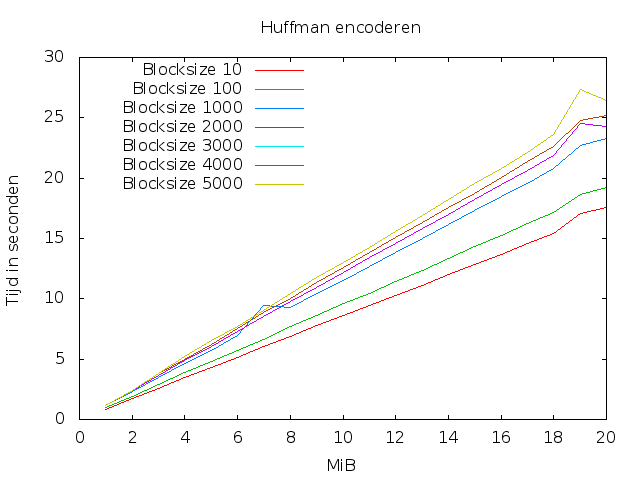
\includegraphics[scale=0.5]{huffman_encoderen.png}
\caption{Uitvoeringstijd voor het encoderen van 20 pseudo random bestanden met een variabele blokgrote.}
\end{figure}
\subsubsection*{Tekst files}
Om de compressie te testen van gewone tekst bestanden heb ik bepaalde RFC teksten gedownload van verschillende grote var\"ierend van 11KiB tot 167Kib. Al deze tekst bestanden heb ik laten comprimeren en terug decomprimeren (om te controleren dat het resultaat van de decompressie nog altijd correct was met het origineel), en ook dit laten uitvoeren voor verschillende blokgrotes, deze keer was de variatie kleiner omdat de bestanden kleiner waren. Voor elk getest bestand was het resultaat een kleiner bestand, hoe groter de blokgrote hoe beter de uiteindelijke compressie was, voor bepaalde blokgrotes was het resultaat 40\% kleiner. Het resultaat de compressie voor rfc 3918 en rfc 1946 vind u hieronder.\\

\includegraphics[scale=0.5]{rfc_compressie1.jpg}\\
\includegraphics[scale=0.5]{rfc_compressie2.jpg}\\

De reden dat hier zoon goeie compressie kan worden bekomen tegenover binaire bestanden (wat we hieronder zullen beschouwen) is dat Burrows-Wheeler en move-to-front echt zeer goed werken op teksten waar er een verband is tussen de opeenvolgende bytes.
\subsubsection*{JPG/MP3 en Binaire files}
In tegenstelling tot mijn verwachtingen comprimeren JPG/MP3 en binaire bestanden niet goed met mijn implementatie van huffman. De reden hiervoor is omdat deze 2 bestandsformaten al zijn gecomprimeerd en er geen redundantie meer aanwezig is die kan worden gebruikt om het bestand nog kleiner te maken.
\begin{figure}[hbt]
\includegraphics[scale=0.5]{audio-compressie.jpg}
\caption{Comprimeren van een 50MB MP3 Audio bestand, we zien voor de laaste 3 blokgrotes een zelfde resultaat, dit is omdat het originele bestand volledig kan worden bevat in de blokgrote.}
\end{figure}
\begin{figure}[hbt]
\includegraphics[scale=0.5]{jpg-compressie.jpg}\\
\pagebreak
\caption{Comprimeren van een JPG-bestand}
\end{figure}
\subsubsection*{Samenvatting en conclusie}
We merken nog enkele interesante dingen op. Als we meerdere test bestanden maken waarin we enkel de zelfde byte herhalen zullen we een zeer goede compressie bekomen, maar de performantie zal zeer sterk dalen. De reden hiervoor is het gebruik van quicksort. Quicksort heeft een slechtste geval van $O(n^{2})$,nl alle gelijke symbolen zullen op het laagste punt in de recursie moeten worden opgelost. Het sorteren van de elementen zal de overhand nemen en de performantie zal zeer slecht zijn.\\

\subsection*{LZ77}
\subsubsection*{Samenvatting en conclusie}
LZ77 is een "Variable-Rate coding" en  maakt gebruikt van een \emph{sliding window} dat wordt gebruikt om een dynamische woordenboek op te bouwen op basis van de te encoderen tekst. Het voordeel hier is dat in tegelstelling tot huffman er geen extra meta informatie moet doorsturen naar de ontvanger.\\

Een nadeel bij dit algoritme is dat het "computation intensive" is, dit komt rechtstreeks door $G$, wat de grote is van het \emph{sliding window}, hoe groter we $G$ maken hoe meer werk het zal zijn een mogelijke langste match te vinden. We merken wel op dat, hoe groter we $G$ maken, hoe beter onze compressie zal zijn.\\

Wat we met LZ77-compresie bekomen is "contextueel comprimeren". Dit is de herkenning dat bepaalde delen van een file een "context" hebben, bv een tekst bestand kan eerst gaan over een onderwerp waar eventueel herhaaldelijk	kan worden gebruikt gemaakt van vakjargon. Of een tekst kan eerst gaan over een zeker onderwerp, endan overgaan tot een ander onderwerp. Het sliding window kunnen we zien als een herkenning dat er een soort van taalkundige lokaliteit is in tekst bestanden.\\

LZ77-compressie zal zeer goed comprimeren voor tekst bestanden en bestanden waarin contextuele lokaliteit aanwezig is. Om dit nog extra uit te buiten pas ik eerst Burrows-Wheeler toe (veel herhalingen die voorkomen in groepen). Een finale opmerking is, hoe groter we $G$ kiezen, hoe beter de compressie zal zijn maar hoe trager het algoritme werkt. Het decoderen kan in lineaire tijd\\

De complexiteit 
Als we de complexiteit beschouwen van LZ77 moeten kijken naar het gebruikte string matching algoritme en de complexiteit van LZ77 zelf.  Voor LZ77 zelf moeten we alle tekens minimaal 1 keer overlopen en per iteratie zoeken achter de langste deelstring. Als we enkel de while-lus bekijken over het aantal tekens:
\begin{lstlisting}
while(index_huidig_element <= len-1){
\end{lstlisting}
Dan zal deze $O(n)$ werk moeten doen, het probleem ligt hem in het string matching algoritme. De complexiteit van het standaard "Knuth-Morris-Pratt"-algoritme is $O(l+k)$, waar $l$ de lengte is van van de zoekstring en $k$ de lengte is van de tekst waarin moet worden gezocht. Dit zal dus leiden tot $O(n(l+k))$ complexiteit. Maar het algoritme is lichtjes aangepast, $l$ is de lengte van mijn \emph{sliding window}, dus $l=G$, $k$ kan in dit geval varieren tot $n-(G+o)$, waar $o$ het aantal bytes is voor de start van het \emph{sliding window}, wat dus gewoon de rest van de string is vanaf het einde van het \emph{sliding window}. Maar dit is niet het geval in mijn implementatie die $G$ als een bovengrens neemt voor $l$, dus resulteert dus in de complexiteit: $O(n(G+G))$, waar $G$ variabel is.
\end{document}